\documentclass[10pt,a4paper,twocolumn]{article}

\usepackage{graphicx}
\usepackage{mathtools}

\begin{document}
\title{A Bayesian Hierarchical Model for Learning Natural Scene Categories}

\author{Li Fei-Fei\\
California Institute of Technology\\ Electrical Engineerig Dept.\\
Pasadena, CA 91125, USA\\
feifeili@vision.caltech.edu \and
Pietro Perona\\
California Institute of Technology\\ Electrical Engineerig Dept.\\
Pasadena, CA 91125, USA\\
perona@vision.caltech.edu}

\maketitle

\begin{abstract}
\hspace{.5cm}We propose a novel approach to learn and recognize natural scene categories. Unlike previous work \cite{oliva, vogel}, it doesnot require experts to annotate the training set. We represent the image of a scene by a collection of local regions, denoted as codewords obtained by unsupervised learning. Each region is represented as part of a “theme”. In previous work, such themes were learnt from hand-annotations of experts, while our method learns the theme distributions as well as the codewords distribution over the themes without supervision. We report satisfactory categorization performances on a large set of 13 categories of complex scenes.
\end{abstract}

\section{Introduction}
\hspace{.5cm}The ability to analyze and classify accurately and rapidly the scene in which we find ourselves is highly useful ineveryday life. Thorpe and colleagues found that humans are able to categorize complex natural scenes containing animals or vehicles very quickly \cite{fize}. Li and colleagues later showed that little or no attention is needed for such rapid natural scene categorization \cite{koch}. Both of these studies posed a serious challenge to the conventional view that to understand the context of a complex scene, one needs first to recognize the objects and then in turn recognize the category of the scene \cite{gelade}.\\

\hspace{.5cm}Can we recognize the context of a scene without having first recognized the objects that are present? A number of recent studies have presented approaches to classify indoor versus outdoor, city versus landscape, sunset versus mountain versus forest using global cues (e.g. power spectrum, color histogram information) \cite{picard, szummer, jain}. Oliva and Torralba further incorporated the idea of using global frequency with local spatial constraints \cite{oliva}. The key idea is to use intermediate representations before classifying scenes: scenes are first labelled with respect to local and global properties by human observers. Similarly, Vogel and Schiele also used an intermediate representation obtained from human observers in learning the semantic context of a scene \cite{vogel}.

\begin{figure}
%\centering
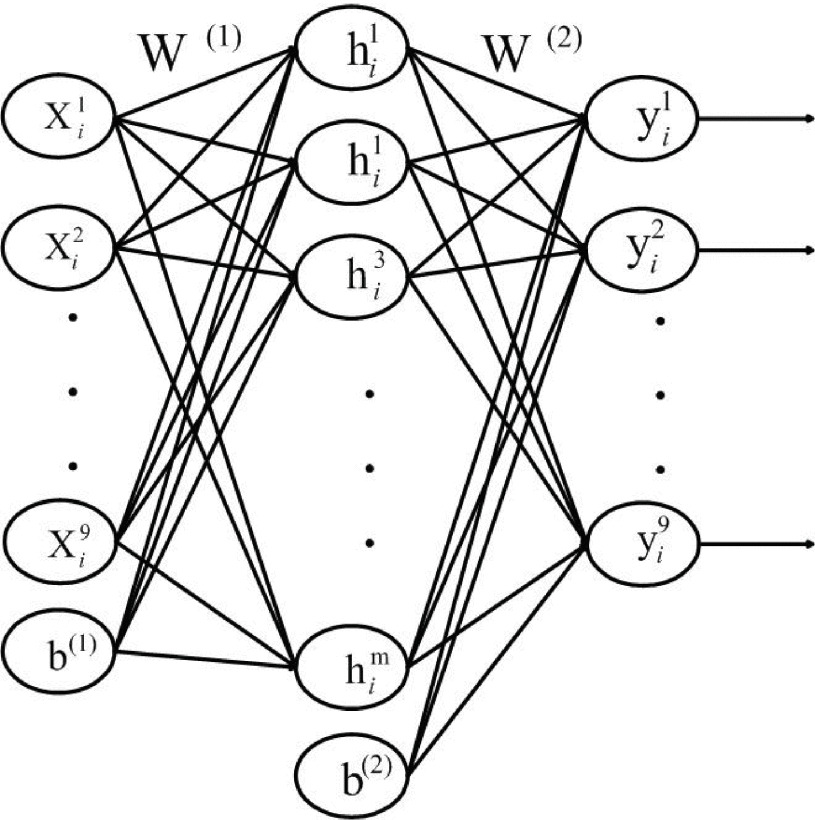
\includegraphics[scale=.3]{figure_1.jpg}
\caption{Our dataset consists of 13 categories, the largest natural scene category dataset to date. Detailed description of the dataset is in Section \ref{secdataset}.}
\label{fig:dataset}
\end{figure}

\hspace{.5cm}A main requirement of such approaches is the manual annotation of “intermediate” properties. In \cite{oliva}, human subjects are instructed to rank each of the hundreds of training scenes into 6 different properties (e.g. ruggedness, expansiveness, roughness, etc). In \cite{vogel}, human subjects are asked to classify 59, 582 local patches from the training images into one of 9 different “semantic concepts” (e.g. water, foliage, sky, etc.). Both cases involve tens of hours of manual labor. These works clearly point to the usefulness of these intermediate representations and motivate us to think of methods for learning such representations directly from the data: both because hand-annotating images is tedious and expensive, and because expert-defined labels are somewhat arbitrary and possibly sub-optimal.\\

\hspace{.5cm}Much can also be learnt from studies for classifying different textures and materials \cite{portilla, malik, varma}. Traditional texture models first identify a large dictionary of useful textons (or codewords). Then for each category of texture, a model is learnt to capture the signature distribution of these textons.
We could loosely think of a texture as one particular intermediate representation of a complex scene. Again, such methods yield a model for this representation through manually segmented training examples. Another limitation of the traditional texture model is the hard assignment of one distribution for a class. This is fine if the underlying images are genuinely created by a single mixture of textons. But his is hardly the case in complex scenes. For example, it is not critical at all that trees must occupy 30\% of a suburb scene and houses 60\%. In fact, one would like to recognize a suburb scene whether there are many trees or just a few.\\

\hspace{.5cm}The key insights of previous work, therefore, appear to be that using intermediate representations improves performance, and that these intermediate representations might be thought of as textures, in turn composed of mixtures of textons, or codewords. Our goal is to take advantage of these
insights, but avoid using manually labeled or segmented images to train the system, if possible at all. To this end, we adapt to the problems of image analysis recent work by Blei and colleagues \cite{blei}, which was designed to represent and learn document models. In this framework, local regions are first clustered into different intermediate themes, and then into categories. Probability distributions of the local regions as well as the intermediate themes are both learnt in an automatic way, bypassing any human annotation. No supervision is needed apart from a single category label to the training image. We summarize our contribution as follows.

\begin{itemize}
\item Our algorithm provides a principled approach to learning relevant intermediate representations of scenes automatically and without supervision.

\item  Our algorithm is a principled probabilistic framework for learning models of textures via codewords (or textons) \cite{malik, portilla, varma}. These approaches, which use histogram models of textons, are a special case of our algorithm. Given the flexibility and hierarchy of our model, such approaches can be easily generalized and extended using our framework.

\item  Our model is able to group categories of images into a sensible hierarchy, similar to what humans would do.
\end{itemize}

We introduce the generative Bayesian hierarchical model for scene categories in Section \ref{approach}. Section \ref{secdataset} describes our dataset of 13 different categories of scenes and the experimental setup. Section \ref{results} illustrates the experimental results. We discuss in Section \ref{summary} our results and future directions.\\

\begin{figure}
%\centering
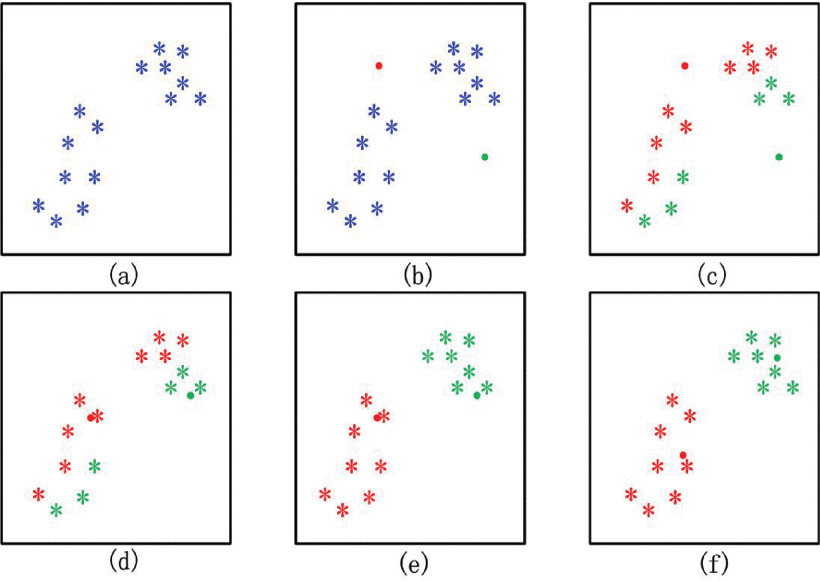
\includegraphics[scale=.2]{figure_2.jpg}
\caption{ Flow chart of the algorithm.}
\label{fig:algo}
\end{figure}

\section{Our Approach} \label{approach}

Fig.\ref{fig:algo} is a summary of our algorithm in both learning and recognition. We model an image as a collection of local patches. Each patch is represented by a codeword from a large vocabulary of codewords (Fig.4). The goal of learning is to achieve a model that best represents the distribution of these codewords in each category of scenes. In recognition, therefore, we first identify all the codewords in the unknown image. Then we find the category model that fits best the distribution of the codewords of the particular image. Our algorithm is modified based on the Latent Dirichlet Allocation (LDA) model proposed by Blei et al. \cite{blei}.\\
\hspace{.5cm}We differ from their model by explicitly introducing a category variable for classification. Furthermore, we propose two variants of the hierarchical model (Fig.3(a) and (b)).

\begin{figure}
%\centering
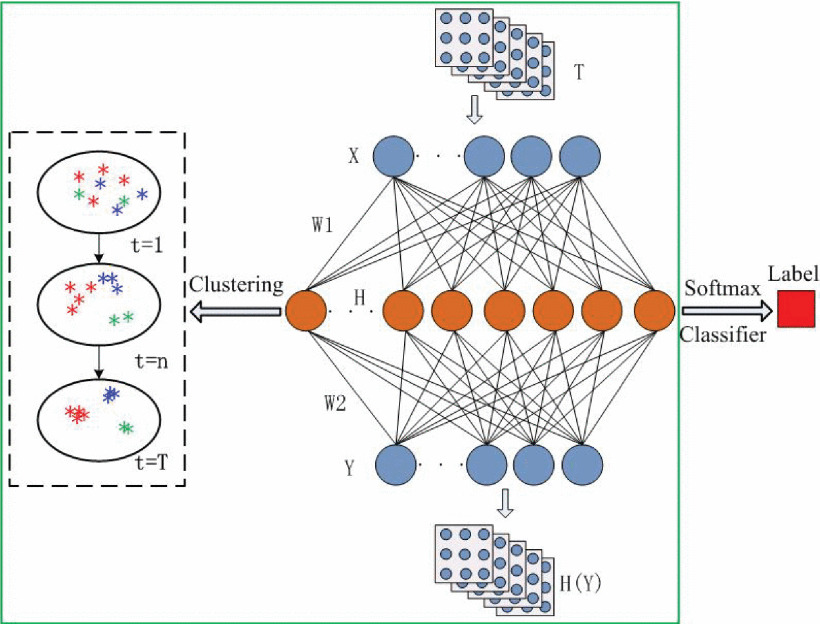
\includegraphics[scale=.1]{figure_3.jpg}
\caption{(a) Theme Model 1 for scene categorization that
shares both the intermediate level themes as well as feature level
codewords. (b) Theme Model 2 for scene categorization that shares
only the feature level codewords; (c) Traditional texton model \cite{malik, varma}.}
\label{fig:three}
\end{figure}

\subsection{Model Structure}
\hspace{.5cm}It is easier to understand the model (Fig.3(a)) by going through the generative process for creating a scene in a specific category. To put the process in plain English, we begin by first choosing a category label, say a mountain scene. Given the mountain class, we draw a probability vector that
will determine what intermediate theme(s) to select while generating each patch of the scene. Now for creating each patch in the image, we first determine a particular theme out of the mixture of possible themes. For example, if a “rock” theme is selected, this will in turn privilege some codewords that occur more frequently in rocks (e.g. slanted lines). Now the theme favoring more horizontal edges is chosen, one can draw a codeword, which is likely to be a horizontal line segment. We repeat the process of drawing both the theme and codeword many times, eventually forming an entire bag of patches that would construct a scene ofmountains. Fig.3(a) is a graphical illustration of the generative model. We will call this model the Theme Model 1. Fig.3(b) is a slight variation of the model in Fig.3(a). We call it the Theme Model 2. Unless otherwise specified, the rest of the paper will focus on Theme Model 1. Now we are ready to show the mathematical details of the formulation of this model and how we learn its parameters.

\subsubsection{The Theme Models}
We begin with some notations and definitions for the Theme Model 1 in Fig.3(a). We will contrast explicitly the use of terminology with both \cite{blei} and the texture studies \cite{malik, varma}.\\

\begin{itemize}
\item  A patch $x$ is the basic unit of an image, defined to be a patch membership from a dictionary of codewords indexed by $\{1, \ldots, T\}$. The $t^{th}$ codeword in the dictionary is represented by a T-vector $x$ such that $x^{t} =1$ and $x^{v} = 0$ for $v \neq t$. In Fig.3(a), $x$ is shaded by common convention to indicate that it is an observed variable. Nodes in the graph that are unobserved have no shading. The equivalent of an image in \cite{blei} is a “document”. And a codeword (or patch) in our model is a “word” in [1]. In texture and material literature, a codeword is also referred as a “texton” \cite{malik, varma}.

\item codeword is also referred as a “texton” \cite{malik, varma}. An image is a sequence of $N$ patches denoted by $x = (x_1, x_2, \ldots, x_N)$, where $x_N$ is the $n^{th}$ patch of the image.

\item A category is a collection of $I$ images denoted by $D = \{x_1, x_2, \ldots, x_I\}$. In \cite{blei}, this is equivalent to a “corpus”.
\end{itemize}

We can now write down the process that generates an image $i$ formally from the model.

\begin{enumerate}

\item hoose a category label $c \sim p(c\mid\eta)$ for each image, where $c = \{1, \ldots, C\}$. C is the total number of categories. $\eta$ is a $C$-dimensional vector of a multinomial distribution;

\item $C$-dimensional vector of a multinomial distribution; Now for this particular image in category $c$, we want to draw a parameter that determines the distribution of the intermediate themes (e.g. how “foliage”, “water”, “sky” etc. are distributed for this scene). This is done by choosing $\pi\sim p(\pi\mid c, \theta)$ for each image. $\pi$ is the parameter of a multinomial distribution for choosing the themes. $\theta$ is a matrix of size $C \times K$, where $\theta_c$ is the $K$-dimensional Dirichlet parameter conditioned on the category $c$. $K$ is the total number of themes.

\item  for each $N$ patches $x_n$ in the image
\begin{itemize}
\item Choose a theme $z_n \sim Mult(\pi)$. $z_n$ is a $K$-dim unit vector. $z_n^{k} = 1$ indicates that the $k^{th}$ theme is selected(e.g. “rock” theme).

\item Choose a patch $x_n \sim p(x_n \mid z_n, \beta)$, where $\beta$ is a matrix of size $K \times T$ . $K$ is again the number of themes and $T$ is the total number of codewords in the codebook. Therefore we have $\beta_{kt} = p(x_t^{n} = 1|z_n^{k} = 1)$.
\end{itemize}
\end{enumerate}

\hspace{.5cm}A $K$−dimensional Dirichlet random variable $π$ has the Kproperty such that $\pi_i \geq 0, \sum_{i=1}^{K} \pi_i = 1$. It is a conjugate distribution of a multinomial distribution. Since the themes $z$ are best described as a discrete variable over the multinomial distribution, Dirichlet distribution becomes the natural choice to describe distribution of $\pi$ \cite{gelman}. It has the following probability density:

\begin{equation}
Dir(\pi \mid \theta_c)= \frac{\Gamma(\sum_{i=1}^{K} \theta_{ci})}{\Pi_{i=1}^{k} \Gamma(\theta_{ci})} \pi_{i}^{(\theta_{ci}-1)}\ldots\pi_{K}^{(\theta_(cK-1)}
\end{equation}

Given the parameters $\theta$, $\eta$ and $\beta$, we can now write the full generative equation of the model. It is the joint probability of a theme mixture $\pi$, a set of $N$ themes $z$, a set of $N$ patches $x$ and the category $c$ is

\begin{equation} \label{eq:fst}
p(x, z, \pi, c \mid \theta, \eta, \beta)=p(c\mid\eta)p(\pi\mid c, \theta)\cdot \Pi_{n=1}^{N}p(z_{n}\mid\pi)p(x_{n}\mid z_{n}, \beta)
\end{equation}
\begin{equation}
p(c\mid\eta)=Mult(c\mid\eta)
\end{equation}
\begin{equation}
p(\pi\mid c, \theta)=\Pi_{j=1}^{C} Dir(\pi\mid\theta_{j})^{\delta(c, j)}
\end{equation}
\begin{equation}
p(z_n\mid\pi)=Mult(z_n\mid\pi)
\end{equation}
\begin{equation}
p(x_n\mid z_n, \beta)= \Pi_{k=1}^K p(x_n\mid\beta_k)^{\delta(z_n^k, 1)}
\end{equation}

As Fig.\ref{fig:three}(a) shows, Theme Model 1 is a hierarchical representation of the scene category model. The Dirichlet parameter $\beta$ for each category is a category-level parameters, sampled once in the process of generating a category of scenes. The multinomial variables $\pi$ are scene-level variables, sampled once per image. Finally, the discrete theme variable $z$ and patch $x$ are patch-level variables, sampled every time a patch is generated.\\
If we wish to model the intermediate themes for each
category without sharing them amongst all categories, we
would introduce a link between the class node $c$ to each
patch $x_n$ , such that $x_n \sim p(xn |zn , β, c)$, where there are $C$
different copies of $\beta$, each of the size $K \times T$ , where $β_{kt}^c=p(x_n^t\mid z_n^k=1)$. The generative equations above (Eq.2-6) are hence changed according to this dependency on c. Due to space limitation, we shall omit deriving the learning and inference rules for this second theme model. We will release a technical note with this paper online for completeness.

\subsubsection{ Bayesian Decision}
Before we show how we could proceed to learn the model parameters, let us first look at how decisions are made given an unknown scene. An unknown image is first represented by a collection of patches, or codewords. We keep the notation $x$ for an image of $N$ patches. Given $x$, we would like to compute the probability of each scene class
\begin{equation}
p(c\vert x, \theta, \beta, \eta)\propto p(x\vert c, \theta, \beta)p(c\vert \eta)\propto p(x\vert c, \theta, \beta)
\end{equation}

where $\theta$, $\beta$ and $\eta$ are parameters learnt from a training set. For convenience, the distribution of $p(c\mid\eta)$ is always assumed to be a fixed uniform distribution in which $p(c)=1/C$. Therefore we will omit to estimate $\eta$ from now on. Then the decision of the category is made by comparing the likelihood of $x$ given each category: $c= arg max cp(x\mid c,\theta,\beta)$. The term $p(x\mid c,0,\beta)$ is in general obtained by integrating over the hidden variables $\pi$ and $z$ in Eq.\ref{eq:fst}.
\begin{equation} \label{eq:krunker}
p(x\vert \theta, \beta, c)=\int p(\pi\vert \theta, c)\left(\prod_{n=1}^{N}\sum_{z_{n}}p(z_{n}\vert \pi)p(x_{n}\vert z_{n}, \beta)\right)d\pi
\end{equation}

Unfortunately Eq.\ref{eq:krunker} is not tractable due to the coupling between $\pi$ and $\beta$ \cite{blei}. However, a wide range of approximate inference algorithms can be considered, including Laplace approximation, variational approximation and MCMC method \cite{blei}. In the following section, we briefly outline the variational method based on Variational Message Passing (VMP) \cite{winn}, a convenient framework to carry out variational inferences.

\subsubsection{Learning: Variational Inference}
In learning, our goal is to maximize the log likelihood term $logp(x\mid\theta, \beta, c)$ by estimating the optimal $\theta$ and $\beta$. Using Jensen's inequality, we can bound this log likelihood in the following way.

\begin{equation}
\begin{split}
\log p(x\mid \theta, \beta)
\geq \int\sum_{z}q(\pi, z)\log p(\pi, z, x\mid \theta, \beta)d\theta \\
\quad\int\sum_{z}q(\pi, z)\log q(\pi, z) \\
=E_{q}[\log p(\pi, z, x\mid \theta, \beta)]-E_{q}[\log q(\pi, z)]
\end{split}
\end{equation}

where $q(\pi,z\mid\gamma,\phi)$ could be any arbitrary variational distribution. By letting $L(\gamma,\phi;\theta,\beta)$ denote the RHS of the above equation, we have:

\begin{equation} \label{eq:qwe}
\begin{split}
\log p(x\vert \theta, \beta) = L(\gamma, \phi;\theta, \beta)+\\
KL(q(\pi, z\vert \gamma, \phi)\vert\vert p(\pi, z\vert x, \theta, \beta))
\end{split}
\end{equation}

where the second term on the RHS of the above equation stands for the Kullback-Leibler distance of two probability densities. By maximizing the lower bound $L(\gamma,\phi;\theta,\theta)$ with respect to $\gamma$ and $\phi$ is the same as minimizing the KL distance between the variational posterior probability and the true posterior probability.\\ 

Given Eq.\ref{eq:qwe}, we first estimate the variational parameters $\gamma$ and $\phi$. Substituting the variational lower bound as a surrogate for the (intractable) marginal likelihood, we can then in turn estimate the model parameters $\theta$ and $\beta$. The iterative algorithm alternates between the following two steps till convergence. We will soon publish a technical note with detailed derivations on our website.

\begin{enumerate}
\item (E-step) For each class of images, optimize values for the variational parameters $\gamma$ and $\phi$. The update rules are
\begin{equation}
\gamma_{i} = \theta_{i}+\sum_{n=1}^{N}\phi_{ni}
\end{equation}
\begin{equation}
\phi_{ni} \propto \beta_{i\nu}\exp\left[\Psi(\gamma_{i})-\Psi(\sum_{j=1}^{K}\gamma_{j})\right]
\end{equation}
where $i$ is the image index, $n$ the patch index and $\Psi(\bullet)$ a digamma function.
\item (M-step) Maximize the reuslting lower bound on the log likelihood with respect to the model parameters $\theta$ and $\beta$. We can do this by finding the maximum likelihood estimates with expected sufficient statistics computed in the E-step \cite{blei}, \cite{minka}.
\end{enumerate}

\subsubsection{A Brief Comparison}
We can compare this hierarchical model with a traditional texton model for texture recognition, for instance \cite{malik, varma}. Fig. \ref{fig:three}(c) is a graphical representation of a traditional texton model. We see here that for a given class of textures or materials, only a single multinomial parameter $\beta$ is associated with the class. In other words, to generate an image, all patches are drawn from a single “theme”. This might be fine when the training data are “pure” textures segmented manually. Since there is no “contaminations” of other “themes”, the single mixture learnt from the codewords might suffice. As shown by [5], this framwork may be further extended by training different models for the same category of textures under different lighting and view point conditions. This again requires manual separations of data and labelling of the segmented textures. In Section \ref{results}, we will show empirically that by explicitly modelling the intermediate themes in these complex scenes, our model achieve better recognition performances than the traditional “texton” model in Fig. \ref{fig:three}(c).

\section{Dataset \& Experimental Setup} \label{secdataset}
\section{Results} \label{results}
\section{Summary \& Discussion} \label{summary}

\begin{thebibliography}{20}

\bibitem{blei}D. Blei, A. Ng, and M. Jordan. Latent dirichlet allocation. Journal of Machine Learning Research, 3:993–1022, 2003.
\bibitem{gelman}A. Gelman, J.B. Carlin, Stern H.S., and Rubin D.B. Bayesian Data Analysis. Chapman Hall/CRC, 1995.
\bibitem{picard}M. Gorkani and R. Picard. Texture orientation for sorting photos at a glance. In Int. Conf. on Pattern Recognition, 1994.
\bibitem{kadir}T. Kadir and M. Brady. Scale, saliency and image description. International Journal of Computer Vision, 45(2):83–105, 2001.
\bibitem{malik}T. Leung and J. Malik. Representing and recognizing the visual appearance of materials using three-dimensional textons. IJCV, 43(1):29–44, June 2001.
\bibitem{koch}F.F. Li, R. VanRullen, C. Koch, and P Perona. Natural scene categorization in the near absence of attention. Proc Natl Acad Sci USA, 99(14):9596–9601, 2002.
\bibitem{lowe}D. Lowe. Object recognition from local scale-invariant features. In Proc. International Conference on Computer Vision, pages 1150–1157, 1999.
\bibitem{minka}T. Minka and J. Lafferty. Expectation-propagation for the generative aspect model. In Proc. of the 18th Conference on Uncertainty in Artificial Intelligence., pages 352–359, 2002.
\bibitem{oliva}A. Oliva and A. Torralba. Modeling the shape of the scene: a holistic representation of the spatial envelope. Int. Journal of Computer Vision., 42, 2001.
\bibitem{portilla}J. Portilla and E.P. Simoncelli. A parametric texture model based on joint statistics of complex wavelet coefficients. IJCV, 40(1):49–70, October 2000.
\bibitem{szummer}M. Szummer and R. Picard. Indoor-outdoor image classification. In Int. Workshop on Content-based Access of Image and Vedeo Databases, Bombay, India, 1998.
\bibitem{fize}S. Thorpe, D. Fize, and C. Marlot. Speed of processing in the human visual system. Nature, 381:520–522, 1996.
\bibitem{murphy}A. Torralba, K. Murphy, and W.T. Freeman. Sharing features: efficient boosting procedures for multiclass object detection. In Proc. of the 2004 IEEE CVPR., 2004.
\bibitem{gelade}A. Treisman and G. Gelade. A feature-integration theory of attention. Cognitive Psychology, 12:97–136, 1980.
\bibitem{jain}A. Vailaya, M. Figueiredo, A. Jain, and H. Zhang. Image classification for content-based indexing. IEEE Trans. on Image Processing. 10, 2001.
\bibitem{varma}M. Varma and A. Zisserman. Texture classification: are filter banks necessary? In CVPR03, pages II: 691–698, 2003.
\bibitem{vogel}J. Vogel and B. Schiele. A semantic typicality measure for natural scene categorization. In DAGM’04 Annual Pattern Recognition Symposium, Tuebingen, Germany, 2004.
\bibitem{winn}J. Winn. Variational Message Passing and its applications. PhD thesis, University of Cambridge, 2003.
\end{thebibliography}

\end{document}